\section{Quicksort e métodos híbridos}
Os algoritmos de ordenação mais utilizados na prática são híbridos, baseados no Quicksort. Tais algoritmos se beneficiam dos pontos positivos do Quicksort ao mesmo tempo em que tentam diminuir o número de movimentações realizadas e evitar o pior caso.

No capítulo anterior, foram apresentados dois algoritmos desse tipo: o QuicksortI, que utiliza a Inserção para finalizar a ordenação, reduzindo o número de movimentações; e o Introsort, algoritmo utilizado na biblioteca padrão da linguagem de programação C\raisebox{0.4ex}{\text{\tiny{++}}}.

O Introsort também utiliza a Inserção para finalizar a ordenação, mas usa o Heapsort quando a árvore de recursão atinge altura igual a $2\log n$, contornando assim os casos em que o Quicksort tende ao pior cenário. O gráfico da Figura \ref{fig:hibridos} a seguir mostra os resultados de tempo e movimentações do Quicksort em comparação com o QuicksortI e o Introsort. Os resultados com relação ao número de comparações foram equivalentes e, por isso, não serão mostrados.

\begin{figure}[H]
\Caption{\label{fig:hibridos}Métodos híbridos – Tempo e movimentações.}
\centering
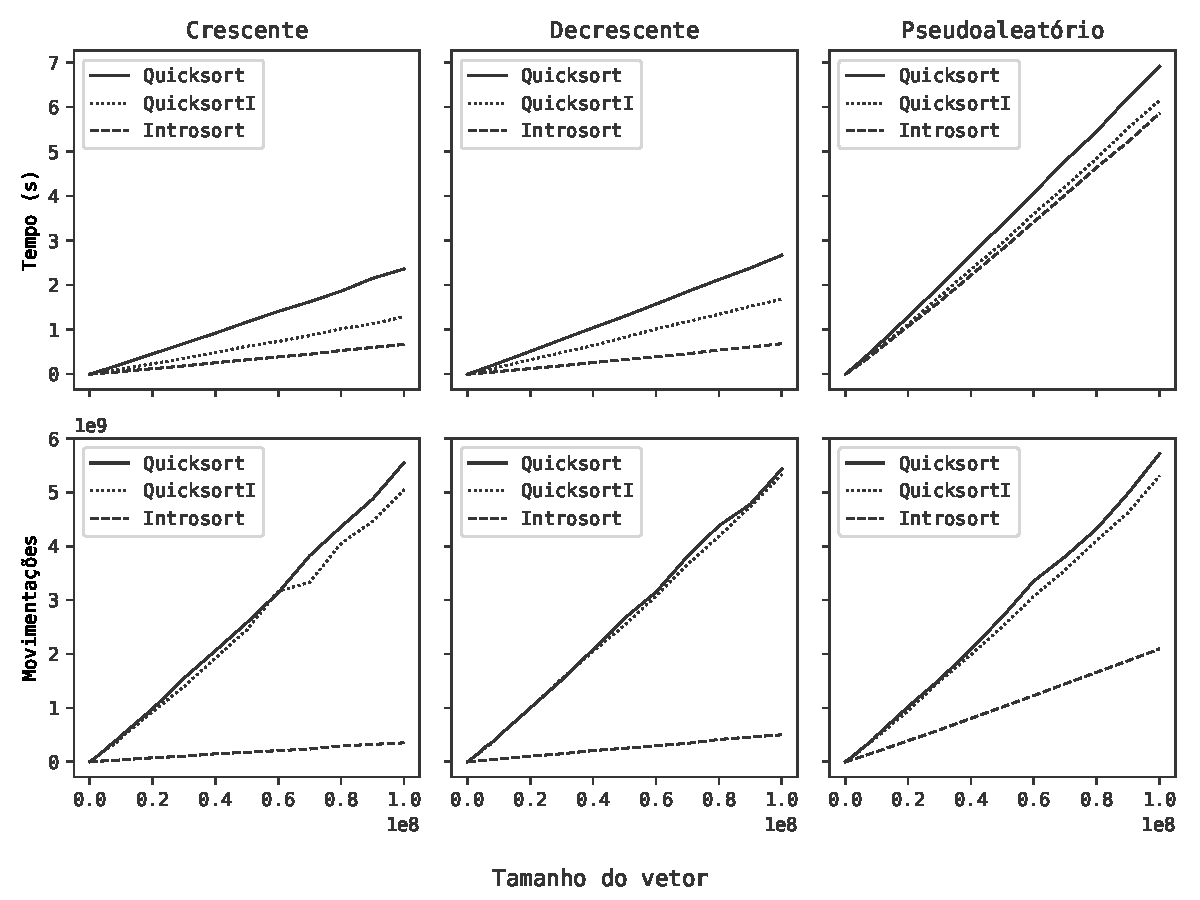
\includegraphics[scale=0.787]{figuras/pdf/hibridos.pdf}
\Fonte{Elaborado pelo autor}
\end{figure}
